%==================================================================================================================================
% COPYRIGHT FG BKS, UNIVERSITY OF KOBLENZ
% Do not change anything. Start in the section where your work starts
%==================================================================================================================================
\documentclass[%
	BCOR=8.25mm,         % Bindekorrektur
	DIV=12,              % Satzspiegel
	parskip=half,		 % Abstand zwischen Absaetzen
	toc=bibliography,	 % Literaturverzeichnis im Inhaltsverzeichnis
	headsepline=on,      % Trennlinie Kolumnentitel
	%twoside,
	oneside,
	toc=listof,
	toc=index,
	enabledeprecatedfontcommands,
	]{scrbook}
\usepackage{mathptmx}
\usepackage{amssymb}
\usepackage{xspace}
\usepackage{color}
\usepackage{subfigure}
\usepackage{amsmath}
\usepackage{amsthm}
\usepackage{float}
\usepackage{url}
\usepackage{tikz}
\usepackage{wasysym} 				 	% fuer die Checkboxen
\usepackage[onehalfspacing]{setspace} 	% Zeilenabstand 
\usepackage{layout}						% Seitenabstaende
\usepackage{fancyhdr}					% Header
\usepackage{lipsum}						% filling Text
\usepackage{natbib} 					% Literaturverzeichnis
\usepackage[english, ngerman]{babel} 	% deutsche typogr. Regeln + Trenntabelle
\usepackage[T1]{fontenc}             	% interner TeX-Font-Codierung
%\usepackage{lmodern}                 	% Font Latin Modern
\usepackage[utf8]{inputenc}          	% Font-Codierung der Eingabedatei
%\usepackage{fontspec}					% lokale Schriftarte

%\setmainfont{Cambria}				
%\setsansfont{Calibri}

\usepackage[babel]{csquotes}         	% Anfuehrungszeichen
\usepackage{graphicx}                	% Graphiken
\usepackage{booktabs}                	% Tabellen schoener
\usepackage{listingsutf8}            	% Listings mit Einstellungen
%\usepackage{titlesec}					% Aendern der Ueberschriften
\usepackage[						 	% Bildunterschrift mit globaler definition
	labelfont=bf,
	font=small
	]{caption}

%% \CharacterTable
%%  {Upper-case    \A\B\C\D\E\F\G\H\I\J\K\L\M\N\O\P\Q\R\S\T\U\V\W\X\Y\Z
%%   Lower-case    \a\b\c\d\e\f\g\h\i\j\k\l\m\n\o\p\q\r\s\t\u\v\w\x\y\z
%%   Digits        \0\1\2\3\4\5\6\7\8\9
%%   Exclamation   \!     Double quote  \"     Hash (number) \#
%%   Dollar        \$     Percent       \%     Ampersand     \&
%%   Acute accent  \'     Left paren    \(     Right paren   \)
%%   Asterisk      \*     Plus          \+     Comma         \,
%%   Minus         \-     Point         \.     Solidus       \/
%%   Colon         \:     Semicolon     \;     Less than     \<
%%   Equals        \=     Greater than  \>     Question mark \?
%%   Commercial at \@     Left bracket  \[     Backslash     \\
%%   Right bracket \]     Circumflex    \^     Underscore    \_
%%   Grave accent  \`     Left brace    \{     Vertical bar  \|
%%   Right brace   \}     Tilde         \~}


\lstset{basicstyle=\small,
	tabsize=2,
	basewidth={0.5em,0.45em},
	extendedchars=true}
\usepackage{amsmath}	               % Mathematik
\usepackage{hyperref}       
\hypersetup{
	bookmarksopen=true,
	bookmarksopenlevel=3,
	citecolor=black,
	linkcolor=black
}

\usepackage{scrhack}				% unterdrueckt Fehlermeldung von listings

%% Verzeichnisse
\usepackage{tocstyle} 
\usetocstyle{KOMAlike}
\KOMAoptions{open=any}


%% Nummerierungstiefen
\setcounter{tocdepth}{3}             % 3 Stufen im Inhaltsverzeichnis
\setcounter{secnumdepth}{3} 		     % 3 Stufen in Abschnittnummerierung

%% Seitenabstaende

\setlength{\footskip}{40pt}
\usepackage[
  top=25mm,
  bottom=20mm,
  left=30mm,
  right=30mm,
  asymmetric,
  %oneside,
]{geometry}

%% Header
\fancypagestyle{plain}{%
  \fancyhf{}%
  \fancyhead[R]{\thepage}
  \fancyhead[L]{\rightmark}
  %\fancyhead[RO,LE]{\thepage}
  %\fancyhead[LO]{\leftmark}
  %\fancyhead[RE]{\rightmark}
}
\renewcommand{\chapterheadstartvskip}{\vspace*{1\baselineskip}} %resetting upper margin

%%Bibliography
\bibliographystyle{agsm} % Harvard Stil

%%Fonts
%\renewcommand{\rmdefault}{Cambria}
%\sffamily

%%TODO
\newcommand\TODO[1]{\textcolor{magenta}{\framebox{todo:} #1}}

%%More Citations
\providecommand{\citeTwo}[4]{\citep[{\citealp[#1]{#2};}][#3]{#4}} 
\providecommand{\citeThree}[6]{\citep[{\citealp[#1]{#2}; \citealp[#3]{#4};}][#5]{#6}} 
\providecommand{\citeFour}[8]{\citep[{\citealp[#1]{#2}; \citealp[#3]{#4}; \citealp[#5]{#6};}][#7]{#8}}
 %%% DO NOT CHANGE THIS FILE

%==================================================================================================================================
\begin{document}
%==================================================================================================================================


%==================================================================================================================================
%% Title Page
%==================================================================================================================================
\begin{titlepage}
	
\includegraphics[height=30pt]{img/logo-uni-rot}
	\hfill
	
\includegraphics[height=30pt]{img/logo-iwvi-rot}

	\begin{center}
	\vspace{2.5cm}	
	
	\huge\textbf{\sffamily Titel der Arbeit} %%% TODO: HIER DEN TITEL EINTRAGEN
	\\ \normalsize \TODO{Datei \"offnen und Todos erledigen: inc/Titelseite.tex} %%% LOE–SCHEN
	
	\vspace{2cm}

	%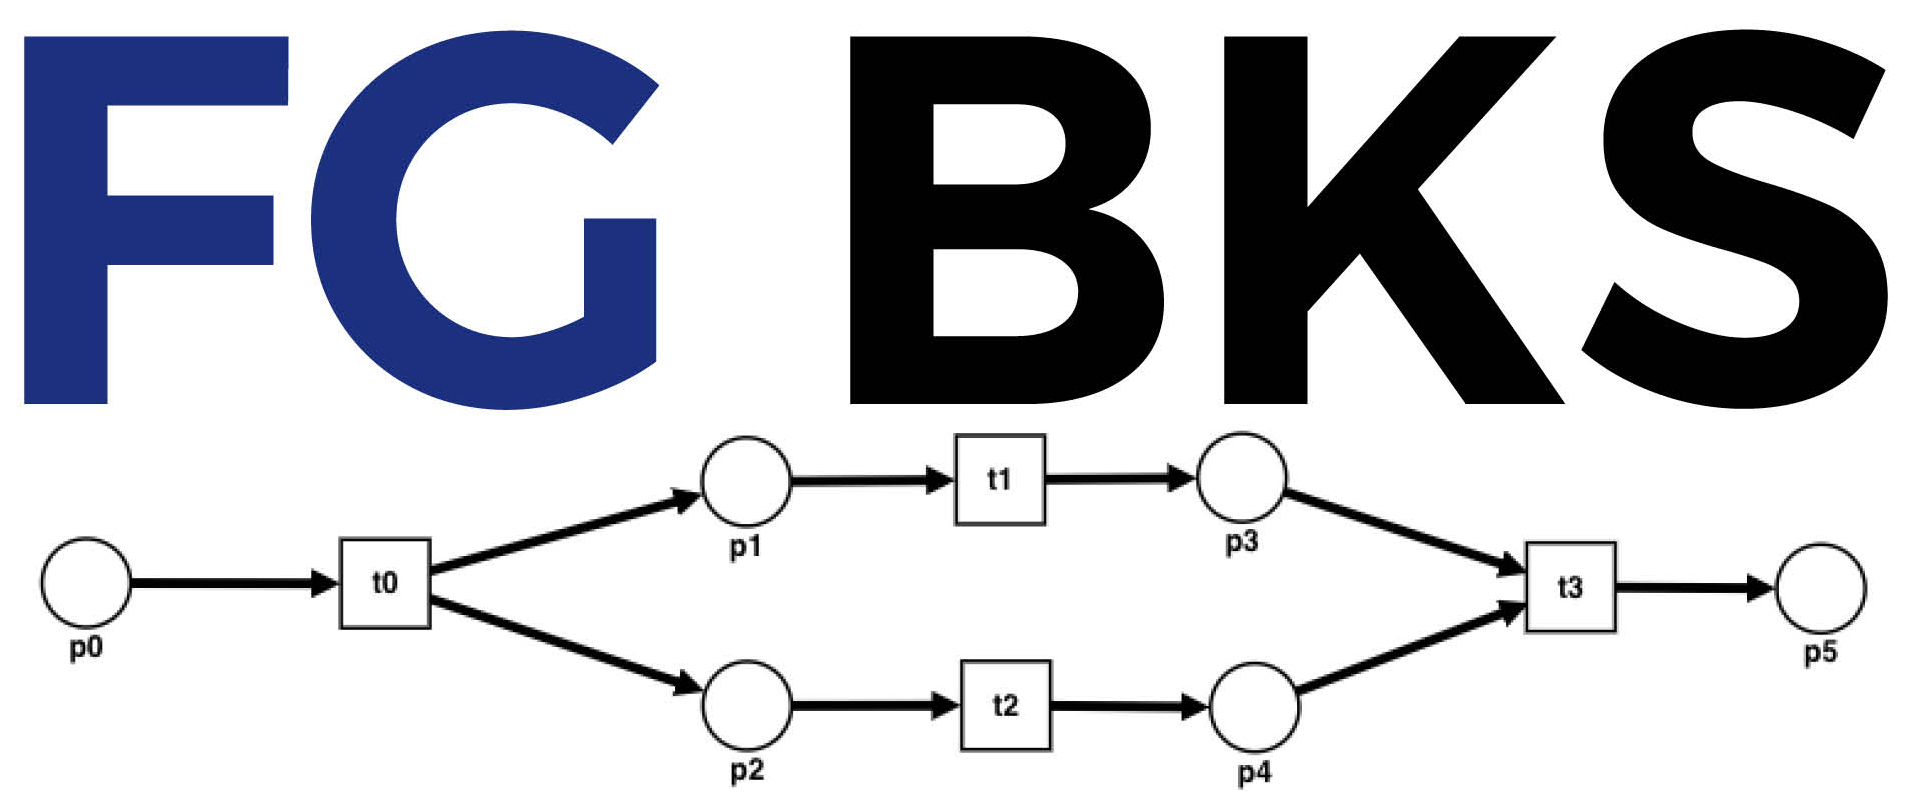
\includegraphics[width=0.3\textwidth]{img/logo-bks}

	\normalsize
	\vspace{1.5cm}	

	\textsc{\Large Seminararbeit | Bachelorarbeit/Masterarbeit}\\Zur Veranstaltung | Zur Erlangung des Grades eines Bachelor/Master of Science im Studiengang Wirtschaftsinformatik/Informationsmanagement\\[2cm] %%% TODO: HIER ZUTREFFENDES AUSWAEHLEN UND REST LOESCHEN
		
	vorgelegt von\\
	
	\textbf{\Large Vorname Name}\\ $ [ $123 456 789$ ] $\\ [1.5cm] %%% TODO: HIER NAME UND MATRIKEL NUMMER EINTRAGEN
	Koblenz, im Monat 202x %%% TODO: HIER MONAT UND JAHR EINTRAGEN
	\end{center}
	\vfill
	\begin{tabular}{ll}
		Erstgutachter: & Prof. Dr. Patrick Delfmann\\ %%% TODO: HIER ERSTGUTACHTER EINTRAGEN
		 & \small{(Institut f\"ur Wirtschafts- und Verwaltungsinformatik, FG Delfmann)}\\
		Zweitgutachter: & Max Mustermann, M.Sc. \\ %%% TODO: HIER ZWEITGUTACHTER EINTRAGEN
		 & \small{(Institut f\"ur Wirtschafts- und Verwaltungsinformatik, FG Delfmann)}\\
		Betreuer:  & Max Mustermann, M.Sc. %%% TODO: HIER BETREUER EINTRAGEN
	\end{tabular}
\end{titlepage}
%\cleardoubleemptypageas

%==================================================================================================================================


%==================================================================================================================================
%% Decleration: DO NOT CHANGE
%==================================================================================================================================
%%%%%%%%%%%%%%%%%%%%
% Diese Datei darf NICHT gaendert werden
% (c) FG BKS, Universitaet Koblenz-Landau
%%%%%%%%%%%%%%%%%%%%

%% Erklaerung
\pagestyle{empty}
\begin{quote}
	\textbf{\Large\sffamily Eidesstattliche Erkl\"arung}

	Hiermit best\"atige ich, dass die vorliegende Arbeit von mir selbst\"andig verfasst wurde und ich keine anderen als die angegebenen Hilfsmittel - insbesondere keine im Quellenverzeichnis nicht benannten Internet-Quellen - benutzt habe und die Arbeit von mir vorher nicht in einem anderen Pr\"ufungsverfahren eingereicht wurde. Die eingereichte schriftliche Fassung entspricht der auf dem elektronischen Speichermedium (CD-Rom).

	\vspace{2em}
	$$
	\begin{tabular}{ l c r }
		&  Ja & Nein \\
		Mit der Einstellung der Arbeit in die Bibliothek bin ich einverstanden. & \Square & \Square\\
		Der Ver\"offentlichung dieser Arbeit im Internet stimme ich zu. & \Square & \Square
	\end{tabular}
	$$

	\vspace{5em}

	\begin{tikzpicture}
		\draw [dotted] (0,0) -- (13,0);
	\end{tikzpicture}
	\\(Ort, Datum) \hspace{3cm} (Unterschrift)
\end{quote}
%\cleardoubleemptypage
%==================================================================================================================================


%==================================================================================================================================
%% Abstract. See file inc/Abstract.tex
%==================================================================================================================================
%%%%%%%%%%%%%%%%%%%%
% Diese Datei muss gaendert werden
% (c) FG BKS, Universitaet Koblenz-Landau
%%%%%%%%%%%%%%%%%%%%




%% Abstract DE
\pagestyle{plain}
\pagenumbering{Roman}
\begin{quote}
	\textbf{\Large\sffamily Zusammenfassung}\\\\
	\TODO{Abstract auf Deutsch schreiben: inc/Abstract.tex}
	\lipsum[1-3] %%% LÃOESCHEN
\end{quote}
\newpage
%\cleardoubleemptypage





%% Abstract EN
\begin{quote}
	\textbf{\Large\sffamily Abstract}\\\\
	\TODO{Abstract auf Englisch schreiben: inc/Abstract.tex}
	\lipsum[1-3] %%% LOE–SCHEN
\end{quote}
%\cleardoubleemptypage

%==================================================================================================================================


%==================================================================================================================================
%% Verzeichnissse
%==================================================================================================================================
\settocfeature{entryhook}{\sffamily}    % alle Eintraege wie im Text serifenlos
\tableofcontents
\settocfeature{entryhook}{\rmfamily}    % Eintraege wie im Text mit Serifen
\listoffigures
\listoftables
%==================================================================================================================================


%==================================================================================================================================
%% Abkuerzungsverzeichnis
%==================================================================================================================================
\addchap[Abk\"uurzungsverzeichnis]{Abk\"urzungsverzeichnis} 
\TODO{Abk\"uzungsverzeichnis bef\"ullen: inc/Glossary.tex}\\
\renewcommand{\arraystretch}{1.5} 
HPA \dotfill Hochschulpr\"ufungsamt\\
z.B. \dotfill zum Beispiel\\
\renewcommand{\arraystretch}{1} 

%\cleardoubleemptypage
\newpage
%==================================================================================================================================


%SETTINGS
\pagestyle{plain}
\pagenumbering{arabic}


%==================================================================================================================================
%==================================================================================================================================
%% YOUR WORK STARTS HERE
%==================================================================================================================================
%==================================================================================================================================


%==================================================================================================================================
\chapter{Vorgaben}
Das Schreiben wissenschaftlicher Arbeiten ist das zentrale Element der universit\"aren Ausbildung im Allgemeinen und somit auch zentrales Element für das Studium. Hiermit werden Sie dazu bef\"ahigt, komplexen Fragestellungen mittels eines konzeptionellen, analytischen Vorgehens beizukommen. 


%==================================================================================================================================
\section{Abgabe und Plagiate}
Bei der Abgabe m\"usen die Vorgaben des Hochschulpr\"ufungsamtes (HPA) beachtet werden: \url{https://www.uni-koblenz-landau.de/de/uni/organisation/verwaltung/abteilungen/abt-3/hsp-ko/dokumente/Merkblatt_Abschlussarbeiten-FB4}. Auch die Informationen zur Anmeldungen und Abgabe des Fachbereiches sind unbedingt zu lesen und einzuhalten: \url{https://www.uni-koblenz-landau.de/de/koblenz/fb4/studierende/pruefungswesen/Abschlussarbeiten}.\\ \\
\textbf{Plagiate} \textit{werden} in der Wissenschaft und demzufolge auch bei Abschlussarbeiten als T\"auschung gewertet. Auch wenn eine T\"auschung erst nach Aush\"andigung des Zeugnisses erkannt wird, kann die Universit\"at die Abschlussarbeit als ``nicht bestanden`` bewerten und das Zeugnis sowie die Bachelor-/Masterurkunde wieder einziehen (§28 der ``Prüfungsordnung Bachelor und Master Fachbereich Informatik``). Achten Sie deshalb auf die korrekte Referenzierung.


\section{Papier- und Seitenformat}
\textbf{Papier:} Es ist lediglich einseitig beschriebenes DIN A 4 mit max. 100g/$m^2$ zul\"assig.\\
\textbf{Schrift:} Der Text ist in Schriftgr\"o{\ss}e 12 Punkt zu verfassen und in Blocksatz zu setzen, \"Uberschriften können durch gr\"o{\ss}ere Schriftgrade bis 16 Punkt hervorgehoben werden. Die Schriftart sind im Dokumenz vorgegeben und dürfen nur in Rücksprache mit dem Betreuer geändert werden. Nehmen Sie von der manuellen Silbentrennung Gebrauch. \\
\textbf{Zeilenabstand:} Der Text ist im 1,5-zeiligem Abstand zu schreiben, \"Uberschriften k\"onnen durch gr\"o{\ss}ere Abst\"ande hervorgehoben werden.\\
\textbf{Randbreite:} Der obere Rand beträgt 2,5 cm, der untere 2 cm. Auf der rechten Seite ist ein Korrekturrand von 3 cm frei zu lassen, der linke Rand sollte dann 3 cm betragen.


\section{Zitate}
Die Verwendung von fremdem geistigem Eigentum ist eindeutig zu kennzeichnen. Dies betrifft sowohl das w\"ortliche Zitat wie auch eine sinngem\"a{\ss}e \"Ubernahme. \\
Die Kennzeichnung erfolgt durch das sog. \textbf{Harvard-System}, also durch Nennung des Verfassers innerhalb des Textes in Klammern (). Erlaubt ist auch die Verwendung des \textbf{APA-Systems} (> v6).\\
Zu nennen ist immer der Autor, das Erscheinungsjahr der Quelle sowie die Seitenzahl (-en) der die Aussage entnommen wurde. Also: (vgl. \citealt[S. 227-228]{corea2017detecting}; vgl. \citealt[S.120]{Delfmann2015DMQL}) \\
Unterschieden wird bei der Referenz im Text zwischen 

\begin{itemize}
	%\item{ der einfachen Nennung im Flie{\ss}text: \citet[S. 120]{Delfmann2015DMQL}},
	\item{ der einfachen Nennung im Flie{\ss}text: \cite[S. 120]{Delfmann2015DMQL}},
	\item einem wörtlichen Zitat: \citep[vgl.][S. 120]{Delfmann2015DMQL},
	\item einer Paraphrase: \citep[vgl.][S. 120]{Delfmann2015DMQL},
	\item und einem Kurzbeleg \citep[S. 120]{Delfmann2015DMQL},
\end{itemize}

wobei Letzteres von einem schlechten wissenschaftlichen Stil zeugt. In Abbildung \ref{fig:zitatformen} sehen Sie die Wichtigsten der aufgezählten Arten mit einem Beispiel.\\
\begin{figure}[h!]
	\centering
	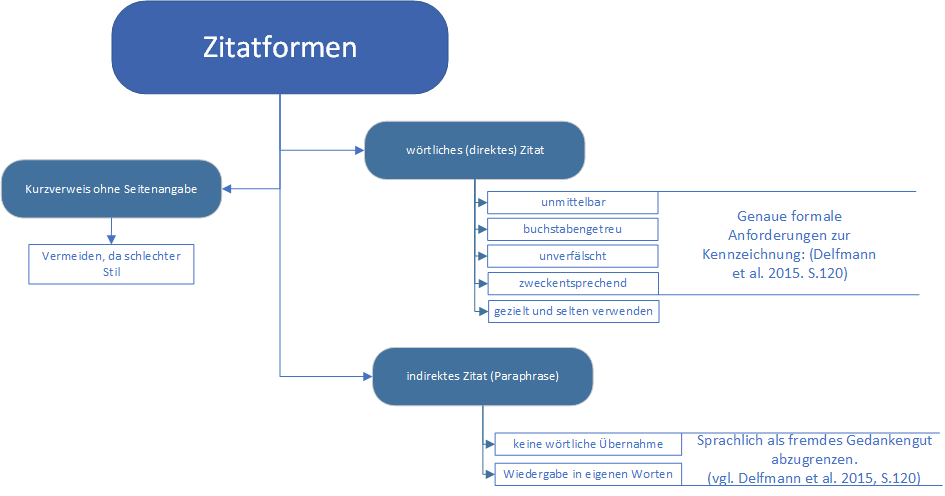
\includegraphics[width=1\textwidth]{img/Zitatformen}
	%\caption{\"Ubersicht der Zitatformen (Quelle: Eigene Darstellung in Anlehnung an \citet[S. 89]{prexl2016digitalen})}
	\caption{\"Ubersicht der Zitatformen (Quelle: Eigene Darstellung in Anlehnung an \cite[S. 89]{prexl2016digitalen})}
	\label{fig:zitatformen}
\end{figure}

Mehrere Quellen werden sortiert (alphabetisch oder chronologisch, wobei ei-ne chronologische Sortierung zu bevorzugen ist – hier werden die aktuellen Quellen zuerst genannt).\\
Die Zitierweise mit Fußnoten ist nicht zul\"assig! Fußnoten dienen ausschlie{\ss}lich der Aufnahme von Randbemerkungen.\\
Das Setzen solcher \textbf{sprechenden Fußnoten} zeugt von Verst\"andnis für das sachgerechte und zielorientierte Schreiben einer wissenschaftlichen Arbeit.\\
W\"ortliche Zitate sind grunds\"atzlich zu vermeiden. Falls es sich um eine Definition handelt, die Ihrer Annahme nach w\"ortlich wiedergegeben werden muss, so setzen Sie diese in Anf\"uhrungszeichen. \"Anderungen des Quellentextes sind dabei kenntlich zu machen. Auslassungen sind durch drei eingeklammerte Punkte anzuzeigen.\\
Wird in einer Arbeit mehr als eine \textbf{Ver\"offentlichung desselben Autors aus einem Jahr} zitiert, m\"ussen die Ver\"offentlichungen durch alphabetische Erweiterung eindeutig gekennzeichnet werden, also z.B. 

\begin{itemize}
	%\item \citep[vgl.][S. 120]{delfmann2015GMQL}
	%\item \citep[vgl.][S. 120]{Delfmann2015DMQL}
	\item \cite[vgl.][S. 130]{Delfmann2015DMQL} 
	\item \cite[vgl.][S. 500]{Delfmann2015GMQL}
\end{itemize}
\textbf{Alle Tabellen und Abbildungen} sind selbst anzufertigen (also keine kopierten/eingescannten Darstellungen verwenden), es sei denn, es handelt sich um Fotografien. \\
Unterhalb von \textbf{Tabellen und Abbildungen} sind diese mit: ``Quelle`` { zu} bezeichnen, ist die Abbildung abgewandelt mit: ``Quelle: eigene Darstellung in Anlehnung an ...``). Ist die Darstellung vollkommen selbst erstellt, so wird sie mit „eigene Darstellung“ gekennzeichnet. Bei der Verwendung von Tabellen und Abbildungen ist stets darauf zu achten, dass im Text Bezug hierzu genommen wird.\\
\textbf{Eigene Tabellen und Abbildungen} m\"ussen als solche gekennzeichnet werden: ``Quelle: eigene Darstellung``.

%==================================================================================================================================
%%% Bibliography 
% Change .bib-file and compile with 'bibtex Vorlage_FG-BKS' in console. Change parameter according to this file name.
%==================================================================================================================================
%\nocite{*} %print all entries
\bibliography{references}{}
%\printbibliography 
%==================================================================================================================================
\end{document}
